\documentclass[]{article}
\usepackage{lmodern}
\usepackage{amssymb,amsmath}
\usepackage{ifxetex,ifluatex}
\usepackage{fixltx2e} % provides \textsubscript
\ifnum 0\ifxetex 1\fi\ifluatex 1\fi=0 % if pdftex
  \usepackage[T1]{fontenc}
  \usepackage[utf8]{inputenc}
\else % if luatex or xelatex
  \ifxetex
    \usepackage{mathspec}
  \else
    \usepackage{fontspec}
  \fi
  \defaultfontfeatures{Ligatures=TeX,Scale=MatchLowercase}
\fi
% use upquote if available, for straight quotes in verbatim environments
\IfFileExists{upquote.sty}{\usepackage{upquote}}{}
% use microtype if available
\IfFileExists{microtype.sty}{%
\usepackage{microtype}
\UseMicrotypeSet[protrusion]{basicmath} % disable protrusion for tt fonts
}{}
\usepackage[margin=1in]{geometry}
\usepackage{hyperref}
\hypersetup{unicode=true,
            pdftitle={Hands on Assessment: Graphs},
            pdfauthor={Paige Dubelko},
            pdfborder={0 0 0},
            breaklinks=true}
\urlstyle{same}  % don't use monospace font for urls
\usepackage{color}
\usepackage{fancyvrb}
\newcommand{\VerbBar}{|}
\newcommand{\VERB}{\Verb[commandchars=\\\{\}]}
\DefineVerbatimEnvironment{Highlighting}{Verbatim}{commandchars=\\\{\}}
% Add ',fontsize=\small' for more characters per line
\usepackage{framed}
\definecolor{shadecolor}{RGB}{248,248,248}
\newenvironment{Shaded}{\begin{snugshade}}{\end{snugshade}}
\newcommand{\KeywordTok}[1]{\textcolor[rgb]{0.13,0.29,0.53}{\textbf{#1}}}
\newcommand{\DataTypeTok}[1]{\textcolor[rgb]{0.13,0.29,0.53}{#1}}
\newcommand{\DecValTok}[1]{\textcolor[rgb]{0.00,0.00,0.81}{#1}}
\newcommand{\BaseNTok}[1]{\textcolor[rgb]{0.00,0.00,0.81}{#1}}
\newcommand{\FloatTok}[1]{\textcolor[rgb]{0.00,0.00,0.81}{#1}}
\newcommand{\ConstantTok}[1]{\textcolor[rgb]{0.00,0.00,0.00}{#1}}
\newcommand{\CharTok}[1]{\textcolor[rgb]{0.31,0.60,0.02}{#1}}
\newcommand{\SpecialCharTok}[1]{\textcolor[rgb]{0.00,0.00,0.00}{#1}}
\newcommand{\StringTok}[1]{\textcolor[rgb]{0.31,0.60,0.02}{#1}}
\newcommand{\VerbatimStringTok}[1]{\textcolor[rgb]{0.31,0.60,0.02}{#1}}
\newcommand{\SpecialStringTok}[1]{\textcolor[rgb]{0.31,0.60,0.02}{#1}}
\newcommand{\ImportTok}[1]{#1}
\newcommand{\CommentTok}[1]{\textcolor[rgb]{0.56,0.35,0.01}{\textit{#1}}}
\newcommand{\DocumentationTok}[1]{\textcolor[rgb]{0.56,0.35,0.01}{\textbf{\textit{#1}}}}
\newcommand{\AnnotationTok}[1]{\textcolor[rgb]{0.56,0.35,0.01}{\textbf{\textit{#1}}}}
\newcommand{\CommentVarTok}[1]{\textcolor[rgb]{0.56,0.35,0.01}{\textbf{\textit{#1}}}}
\newcommand{\OtherTok}[1]{\textcolor[rgb]{0.56,0.35,0.01}{#1}}
\newcommand{\FunctionTok}[1]{\textcolor[rgb]{0.00,0.00,0.00}{#1}}
\newcommand{\VariableTok}[1]{\textcolor[rgb]{0.00,0.00,0.00}{#1}}
\newcommand{\ControlFlowTok}[1]{\textcolor[rgb]{0.13,0.29,0.53}{\textbf{#1}}}
\newcommand{\OperatorTok}[1]{\textcolor[rgb]{0.81,0.36,0.00}{\textbf{#1}}}
\newcommand{\BuiltInTok}[1]{#1}
\newcommand{\ExtensionTok}[1]{#1}
\newcommand{\PreprocessorTok}[1]{\textcolor[rgb]{0.56,0.35,0.01}{\textit{#1}}}
\newcommand{\AttributeTok}[1]{\textcolor[rgb]{0.77,0.63,0.00}{#1}}
\newcommand{\RegionMarkerTok}[1]{#1}
\newcommand{\InformationTok}[1]{\textcolor[rgb]{0.56,0.35,0.01}{\textbf{\textit{#1}}}}
\newcommand{\WarningTok}[1]{\textcolor[rgb]{0.56,0.35,0.01}{\textbf{\textit{#1}}}}
\newcommand{\AlertTok}[1]{\textcolor[rgb]{0.94,0.16,0.16}{#1}}
\newcommand{\ErrorTok}[1]{\textcolor[rgb]{0.64,0.00,0.00}{\textbf{#1}}}
\newcommand{\NormalTok}[1]{#1}
\usepackage{graphicx,grffile}
\makeatletter
\def\maxwidth{\ifdim\Gin@nat@width>\linewidth\linewidth\else\Gin@nat@width\fi}
\def\maxheight{\ifdim\Gin@nat@height>\textheight\textheight\else\Gin@nat@height\fi}
\makeatother
% Scale images if necessary, so that they will not overflow the page
% margins by default, and it is still possible to overwrite the defaults
% using explicit options in \includegraphics[width, height, ...]{}
\setkeys{Gin}{width=\maxwidth,height=\maxheight,keepaspectratio}
\IfFileExists{parskip.sty}{%
\usepackage{parskip}
}{% else
\setlength{\parindent}{0pt}
\setlength{\parskip}{6pt plus 2pt minus 1pt}
}
\setlength{\emergencystretch}{3em}  % prevent overfull lines
\providecommand{\tightlist}{%
  \setlength{\itemsep}{0pt}\setlength{\parskip}{0pt}}
\setcounter{secnumdepth}{0}
% Redefines (sub)paragraphs to behave more like sections
\ifx\paragraph\undefined\else
\let\oldparagraph\paragraph
\renewcommand{\paragraph}[1]{\oldparagraph{#1}\mbox{}}
\fi
\ifx\subparagraph\undefined\else
\let\oldsubparagraph\subparagraph
\renewcommand{\subparagraph}[1]{\oldsubparagraph{#1}\mbox{}}
\fi

%%% Use protect on footnotes to avoid problems with footnotes in titles
\let\rmarkdownfootnote\footnote%
\def\footnote{\protect\rmarkdownfootnote}

%%% Change title format to be more compact
\usepackage{titling}

% Create subtitle command for use in maketitle
\newcommand{\subtitle}[1]{
  \posttitle{
    \begin{center}\large#1\end{center}
    }
}

\setlength{\droptitle}{-2em}

  \title{Hands on Assessment: Graphs}
    \pretitle{\vspace{\droptitle}\centering\huge}
  \posttitle{\par}
    \author{Paige Dubelko}
    \preauthor{\centering\large\emph}
  \postauthor{\par}
      \predate{\centering\large\emph}
  \postdate{\par}
    \date{January 22, 2019}


\begin{document}
\maketitle

\begin{Shaded}
\begin{Highlighting}[]
\CommentTok{#Whisker plot}
\NormalTok{x <-}\StringTok{ }\KeywordTok{rnorm}\NormalTok{(}\DecValTok{1000}\NormalTok{,}\DecValTok{0}\NormalTok{)}
\KeywordTok{boxplot}\NormalTok{(x)}
\end{Highlighting}
\end{Shaded}

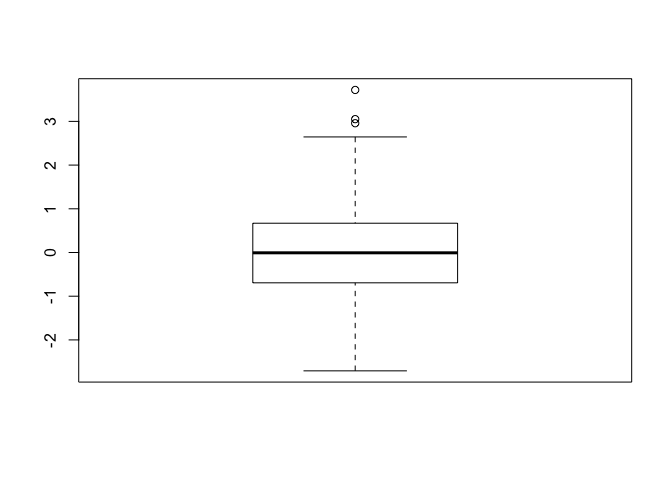
\includegraphics{class05_files/figure-latex/unnamed-chunk-1-1.pdf}

\begin{Shaded}
\begin{Highlighting}[]
\CommentTok{# Age vs Weight - offset graph}
\NormalTok{weight <-}\StringTok{ }\KeywordTok{read.table}\NormalTok{(}\StringTok{"bimm143_05_rstats/weight_chart.txt"}\NormalTok{, }\DataTypeTok{header =} \OtherTok{TRUE}\NormalTok{)}
\KeywordTok{plot}\NormalTok{(weight, }\DataTypeTok{type =} \StringTok{"o"}\NormalTok{, }\DataTypeTok{pch =} \DecValTok{15}\NormalTok{, }\DataTypeTok{cex =} \FloatTok{1.5}\NormalTok{, }\DataTypeTok{lwd =} \DecValTok{2}\NormalTok{, }\DataTypeTok{ylim =} \KeywordTok{c}\NormalTok{(}\DecValTok{2}\NormalTok{,}\DecValTok{10}\NormalTok{),}
     \DataTypeTok{xlab =} \StringTok{"Age (months)"}\NormalTok{, }\DataTypeTok{ylab =} \StringTok{"Weight (kg)"}\NormalTok{,}
     \DataTypeTok{main =} \StringTok{"Baby Weight with Age"}\NormalTok{)}
\end{Highlighting}
\end{Shaded}

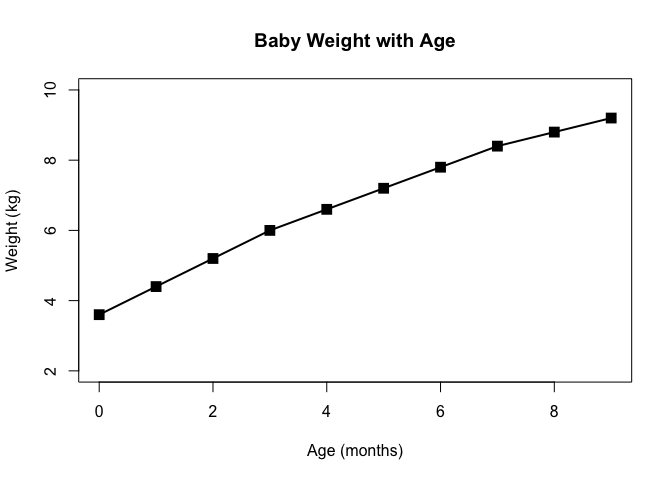
\includegraphics{class05_files/figure-latex/unnamed-chunk-1-2.pdf}

\begin{Shaded}
\begin{Highlighting}[]
\CommentTok{#Bar Graph}
\NormalTok{mouse <-}\StringTok{ }\KeywordTok{read.table}\NormalTok{(}\StringTok{"bimm143_05_rstats/feature_counts.txt"}\NormalTok{, }\DataTypeTok{header =} \OtherTok{TRUE}\NormalTok{,}
                    \DataTypeTok{sep =} \StringTok{"}\CharTok{\textbackslash{}t}\StringTok{"}\NormalTok{)}
\KeywordTok{par}\NormalTok{(}\DataTypeTok{mar =} \KeywordTok{c}\NormalTok{(}\FloatTok{2.5}\NormalTok{,}\DecValTok{11}\NormalTok{,}\DecValTok{2}\NormalTok{,}\DecValTok{2}\NormalTok{))}
\KeywordTok{barplot}\NormalTok{(mouse}\OperatorTok{$}\NormalTok{Count, }\DataTypeTok{main =} \StringTok{"Mouse Genes"}\NormalTok{, }\DataTypeTok{horiz =} \OtherTok{TRUE}\NormalTok{,}
        \DataTypeTok{xlab =} \StringTok{"Count"}\NormalTok{, }\DataTypeTok{names.arg =}\NormalTok{ mouse}\OperatorTok{$}\NormalTok{Feature, }\DataTypeTok{las =} \DecValTok{1}\NormalTok{,}
        \DataTypeTok{col =} \KeywordTok{rainbow}\NormalTok{(}\KeywordTok{nrow}\NormalTok{(mouse)))}
\end{Highlighting}
\end{Shaded}

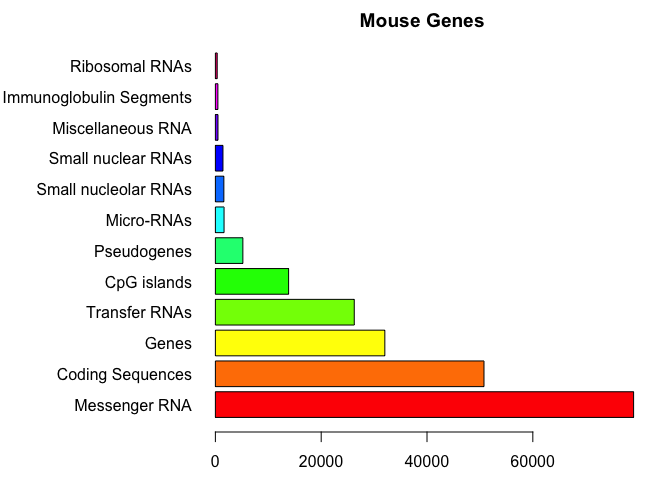
\includegraphics{class05_files/figure-latex/unnamed-chunk-1-3.pdf}

\begin{Shaded}
\begin{Highlighting}[]
\CommentTok{#Histrogram}
\NormalTok{x <-}\StringTok{ }\KeywordTok{c}\NormalTok{(}\KeywordTok{rnorm}\NormalTok{(}\DecValTok{10000}\NormalTok{), }\KeywordTok{rnorm}\NormalTok{(}\DecValTok{10000}\NormalTok{) }\OperatorTok{+}\StringTok{ }\DecValTok{4}\NormalTok{)}
\KeywordTok{hist}\NormalTok{(x, }\DataTypeTok{breaks =} \DecValTok{10}\NormalTok{)}
\end{Highlighting}
\end{Shaded}

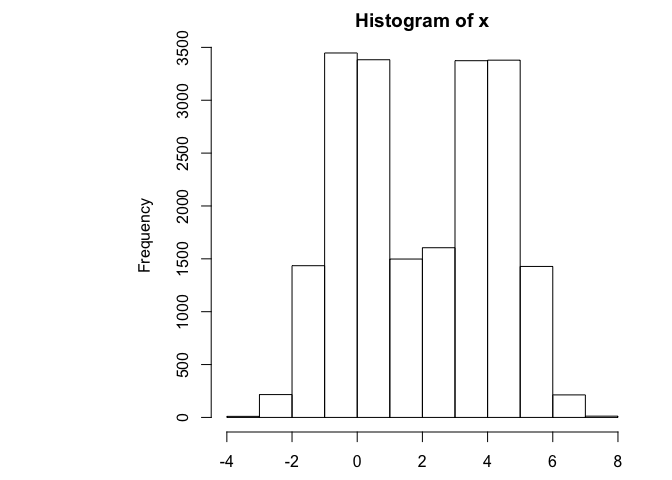
\includegraphics{class05_files/figure-latex/unnamed-chunk-1-4.pdf}

\begin{Shaded}
\begin{Highlighting}[]
\CommentTok{#male_female_counts.txt}
\NormalTok{gender <-}\StringTok{ }\KeywordTok{read.table}\NormalTok{(}\StringTok{"bimm143_05_rstats/male_female_counts.txt"}\NormalTok{, }\DataTypeTok{header =} \OtherTok{TRUE}\NormalTok{,}
                     \DataTypeTok{sep =} \StringTok{"}\CharTok{\textbackslash{}t}\StringTok{"}\NormalTok{)}
\KeywordTok{par}\NormalTok{(}\DataTypeTok{mar =} \KeywordTok{c}\NormalTok{(}\FloatTok{5.1}\NormalTok{,}\DecValTok{5}\NormalTok{,}\DecValTok{5}\NormalTok{,}\FloatTok{2.1}\NormalTok{))}
\KeywordTok{barplot}\NormalTok{(gender}\OperatorTok{$}\NormalTok{Count, }\DataTypeTok{col =} \KeywordTok{c}\NormalTok{(}\StringTok{"blue"}\NormalTok{, }\StringTok{"pink"}\NormalTok{), }\DataTypeTok{main =} \StringTok{"Gender Count"}\NormalTok{,}
        \DataTypeTok{names.arg =}\NormalTok{ gender}\OperatorTok{$}\NormalTok{Sample, }\DataTypeTok{ylim =} \KeywordTok{c}\NormalTok{(}\DecValTok{0}\NormalTok{,}\DecValTok{20}\NormalTok{), }\DataTypeTok{las =} \DecValTok{2}\NormalTok{)}
\end{Highlighting}
\end{Shaded}

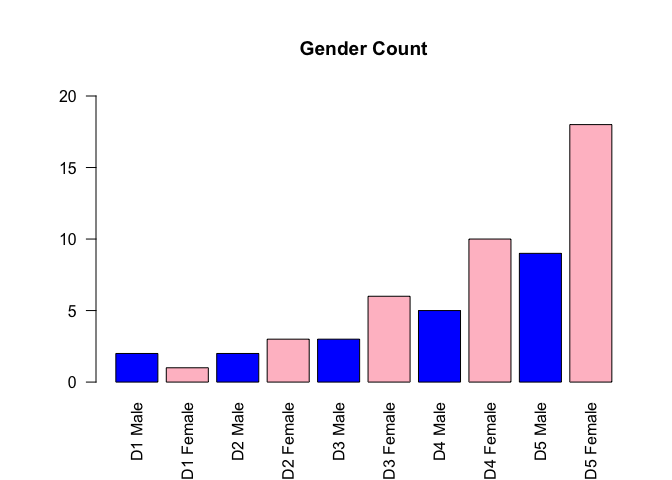
\includegraphics{class05_files/figure-latex/unnamed-chunk-1-5.pdf}

\begin{Shaded}
\begin{Highlighting}[]
\CommentTok{#up_down_expression.txt}
\NormalTok{genes <-}\StringTok{ }\KeywordTok{read.delim}\NormalTok{(}\StringTok{"bimm143_05_rstats/up_down_expression.txt"}\NormalTok{)}
\KeywordTok{palette}\NormalTok{(}\KeywordTok{c}\NormalTok{(}\StringTok{"blue"}\NormalTok{, }\StringTok{"grey"}\NormalTok{, }\StringTok{"magenta"}\NormalTok{))}
\KeywordTok{par}\NormalTok{(}\DataTypeTok{mar =} \KeywordTok{c}\NormalTok{(}\FloatTok{5.1}\NormalTok{,}\DecValTok{5}\NormalTok{,}\DecValTok{5}\NormalTok{,}\FloatTok{2.1}\NormalTok{))}
\KeywordTok{plot}\NormalTok{(genes}\OperatorTok{$}\NormalTok{Condition1, genes}\OperatorTok{$}\NormalTok{Condition2, }\DataTypeTok{col =}\NormalTok{ genes}\OperatorTok{$}\NormalTok{State, }\DataTypeTok{xlab =} \StringTok{"Expression Condition 1"}\NormalTok{,}
     \DataTypeTok{ylab =} \StringTok{"Expression Condition 2"}\NormalTok{, }\DataTypeTok{main =} \StringTok{"Expression Levels"}\NormalTok{)}
\end{Highlighting}
\end{Shaded}

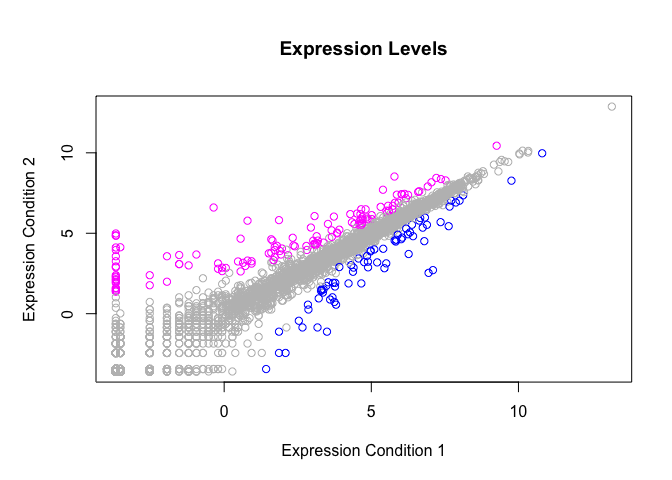
\includegraphics{class05_files/figure-latex/unnamed-chunk-1-6.pdf}

\begin{Shaded}
\begin{Highlighting}[]
\CommentTok{#meth}
\NormalTok{meth <-}\StringTok{ }\KeywordTok{read.delim}\NormalTok{(}\StringTok{"bimm143_05_rstats/expression_methylation.txt"}\NormalTok{)}
\NormalTok{index <-}\StringTok{ }\NormalTok{meth}\OperatorTok{$}\NormalTok{expression }\OperatorTok{>}\StringTok{ }\DecValTok{0}
\NormalTok{color <-}\StringTok{ }\KeywordTok{densCols}\NormalTok{(meth}\OperatorTok{$}\NormalTok{gene.meth[index], meth}\OperatorTok{$}\NormalTok{expression[index],}
                  \DataTypeTok{colramp =} \KeywordTok{colorRampPalette}\NormalTok{(}\KeywordTok{c}\NormalTok{(}\StringTok{"blue"}\NormalTok{, }\StringTok{"green"}\NormalTok{, }\StringTok{"red"}\NormalTok{, }\StringTok{"yellow"}\NormalTok{)))}
\KeywordTok{plot}\NormalTok{(meth}\OperatorTok{$}\NormalTok{gene.meth[index], meth}\OperatorTok{$}\NormalTok{expression[index], }\DataTypeTok{xlab =} \StringTok{"Gene"}\NormalTok{, }\DataTypeTok{ylab =} \StringTok{"Expression"}\NormalTok{,}
     \DataTypeTok{col =}\NormalTok{ color, }\DataTypeTok{pch =} \DecValTok{20}\NormalTok{, }\DataTypeTok{main =} \StringTok{"Gene Expression"}\NormalTok{)}
\end{Highlighting}
\end{Shaded}

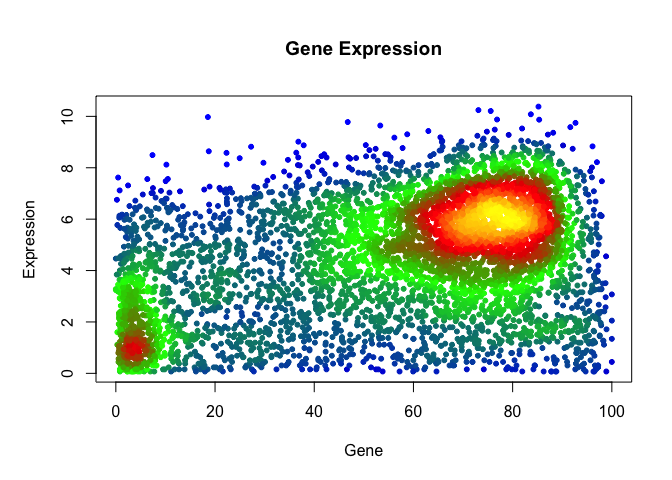
\includegraphics{class05_files/figure-latex/unnamed-chunk-1-7.pdf}


\end{document}
